\documentclass[12pt,a4paper]{article}

% ---------------- Paket ----------------
\usepackage{fontspec}
\setmainfont{TeX Gyre Termes}
\setmonofont{DejaVu Sans Mono}[Scale=MatchLowercase]
\usepackage[a4paper,margin=2.5cm]{geometry}
\usepackage{setspace}
\usepackage{indentfirst}
\usepackage{titlesec}
\usepackage{booktabs}
\usepackage{tabularx}
\usepackage{array}
\usepackage{caption}
\usepackage{enumitem}
\usepackage{tikz}
\usetikzlibrary{arrows.meta,positioning,fit,backgrounds}
\usepackage{xcolor}
% \usepackage{microtype}
\usepackage{fancyhdr}
\usepackage[round]{natbib}
\usepackage[hidelinks]{hyperref}
\usepackage{listings}
\usepackage{url}
\urlstyle{same}
\usepackage{graphicx}

\definecolor{navy}{HTML}{1F3864}
\definecolor{slate}{HTML}{44546A}
\definecolor{lightgray}{HTML}{F2F2F2}
\definecolor{rule}{HTML}{BFBFBF}

\hypersetup{
  pdftitle={POLARIS: Peringatan Dini Berbasis Deception untuk Jaringan IT/OT dengan False Positive Rendah secara Desain},
  pdfauthor={Muh Syahrir Hamdani},
  pdfsubject={Proposal Solusi Kartika Cyber Hackathon 2026},
  pdfkeywords={deception defense, honeytoken, deteksi penyusupan, IT/OT, MITRE ATT&CK, keamanan siber}
}

% ---------------- Format ----------------
\onehalfspacing
\setlength{\parindent}{1.27cm}
\setlength{\parskip}{0pt}
\setlength{\emergencystretch}{3em}

\titleformat{\section}{\normalfont\bfseries\color{navy}\large}{\thesection.}{0.5em}{}
\titlespacing*{\section}{0pt}{14pt}{6pt}
\titleformat{\subsection}{\normalfont\bfseries\color{slate}\normalsize}{\thesubsection}{0.5em}{}
\titlespacing*{\subsection}{0pt}{12pt}{4pt}

\renewcommand{\contentsname}{Daftar Isi}
\renewcommand{\refname}{Daftar Pustaka}
\renewcommand{\tablename}{Tabel}
\renewcommand{\figurename}{Gambar}
\captionsetup[table]{labelsep=space,font=small,labelfont=bf,justification=raggedright,singlelinecheck=false}
\captionsetup[figure]{labelsep=space,font=small,labelfont=bf,justification=centering,singlelinecheck=false}

\pagestyle{fancy}
\fancyhf{}
\renewcommand{\headrulewidth}{0.3pt}
\fancyhead[L]{\footnotesize\textcolor{slate}{POLARIS --- Proposal Solusi}}
\fancyhead[R]{\footnotesize\textcolor{slate}{Kartika Cyber Hackathon 2026}}
\fancyfoot[C]{\thepage}
\fancypagestyle{plain}{\fancyhf{}\fancyfoot[C]{\thepage}\renewcommand{\headrulewidth}{0pt}}

\newcommand{\tabnote}[1]{\par\vspace{2pt}{\footnotesize\textit{Catatan.} #1\par}}

\lstset{
  basicstyle=\ttfamily\footnotesize,
  breaklines=true,
  frame=single,
  rulecolor=\color{rule},
  backgroundcolor=\color{lightgray},
  columns=fullflexible,
  keepspaces=true,
  showstringspaces=false,
  captionpos=b
}

\begin{document}

% ================= HALAMAN JUDUL =================
\begin{titlepage}
\thispagestyle{empty}
\centering
\vspace*{1.0cm}

{\footnotesize\bfseries\color{slate} KARTIKA CYBER HACKATHON 2026}\\[0.15cm]
{\footnotesize\color{slate} Pusat Siber Angkatan Darat (PUSSIBERAD) \(\times\) CODEPOLITAN}\\[1.4cm]

\textcolor{navy}{\rule{\textwidth}{0.8pt}}\\[0.7cm]

{\LARGE\bfseries\color{navy} POLARIS}\\[0.35cm]
{\Large\bfseries Peringatan Dini Berbasis Deception untuk Jaringan IT/OT\\[0.15cm]
dengan False Positive Rendah secara Desain}\\[0.7cm]

{\large Proposal Solusi}\\[0.25cm]
{\large Kategori 02 --- Defensive Shield (Penangkalan)}\\[0.7cm]

\textcolor{navy}{\rule{\textwidth}{0.8pt}}\\[1.3cm]

{\large\bfseries MUH SYAHRIR HAMDANI}\\[0.2cm]
{\normalsize Peserta Individu}\\[1.4cm]

{\normalsize 25 Oktober 2026}\\[0.25cm]
{\small Versi 1.0}

\vfill
{\footnotesize Dokumen ini disusun untuk Babak Penyisihan Online.}\\[0.1cm]
{\footnotesize Batas akhir submission: 15 November 2026.}
\end{titlepage}

% ================= ABSTRAK =================
\section*{Abstrak}
\addcontentsline{toc}{section}{Abstrak}

Pertahanan siber satuan menghadapi dua tekanan yang saling memperkuat: penyusup yang telah melewati perimeter bergerak di dalam jaringan, sementara sistem deteksi berbasis anomali menghasilkan alert dalam jumlah besar dengan false positive yang tinggi. Pada jaringan TNI AD yang sebagian terisolasi dan menggabungkan IT dengan OT/ICS, solusi yang bergantung pada cloud atau threat intelligence eksternal juga sulit diterapkan. Proposal ini merancang POLARIS, sistem peringatan dini berbasis deception yang menanam umpan---decoy port, honeytoken file, canary credential, honeytoken URL, web decoy, dan decoy OT/ICS---yang secara desain tidak dilalui operasi normal. Interaksi dengan umpan diperlakukan sebagai sinyal berkeyakinan tinggi, lalu dikorelasikan menjadi incident, dipetakan ke MITRE ATT\&CK (Enterprise dan ICS), dan diteruskan ke dashboard serta kanal alert. POLARIS dirancang on-prem, dapat berjalan di jaringan air-gap, dan menyediakan bukti yang siap forensik. Penulis menekankan batas klaim: false positive tidak dijamin nol karena backup, pemindai kerentanan, dan kesalahan administrator dapat menyentuh umpan; karena itu proposal ini menyertakan tier kepercayaan, allowlist operasional, dan rencana evaluasi terkontrol. Dokumen ini merupakan proposal solusi dan rencana pengembangan, bukan laporan hasil pengukuran. Target yang akan diuji mencakup latensi deteksi, kelengkapan bukti, jumlah false positive pada beban kerja wajar, dan akurasi korelasi.

\vspace{0.3cm}
\noindent\textit{Kata kunci:} deception defense, honeytoken, deteksi penyusupan, IT/OT, MITRE ATT\&CK, keamanan siber

\vspace{0.7cm}
\section*{Abstract}
\addcontentsline{toc}{section}{Abstract}

Defensive cyber operations face two reinforcing pressures: intruders who have crossed the perimeter move laterally inside the network, while anomaly-based detection systems produce large volumes of alerts with high false-positive rates. In Indonesian Army networks that are partly isolated and combine IT with OT/ICS, solutions depending on cloud services or external threat intelligence are also difficult to deploy. This proposal designs POLARIS, a deception-based early-warning system that plants decoys---decoy ports, honeytoken files, canary credentials, honeytoken URLs, web decoys, and OT/ICS decoys---that normal operations are not expected to touch. Interaction with a decoy is treated as a high-confidence signal, correlated into an incident, mapped to MITRE ATT\&CK (Enterprise and ICS), and delivered to a dashboard and alert channels. POLARIS is designed to run on-premises, operate in air-gapped networks, and preserve forensics-ready evidence. The author states the claim boundary explicitly: false positives are not guaranteed to be zero because backups, vulnerability scanners, and administrator mistakes may touch a decoy; the proposal therefore includes confidence tiers, operational allowlists, and a controlled evaluation plan. This document is a solution proposal and development plan, not a report of measured results. The targets to be tested include detection latency, evidence completeness, false-positive count under a benign workload, and correlation accuracy.

\vspace{0.3cm}
\noindent\textit{Keywords:} deception defense, honeytoken, intrusion detection, IT/OT, MITRE ATT\&CK, cybersecurity

\newpage
\begingroup
\small
\setstretch{1.0}
\tableofcontents
\endgroup
\newpage

% ================= DAFTAR SINGKATAN =================
\section*{Daftar Singkatan}
\addcontentsline{toc}{section}{Daftar Singkatan}

\begin{tabular}{@{}p{0.18\textwidth}p{0.70\textwidth}@{}}
\toprule
\textbf{Singkatan} & \textbf{Kepanjangan} \\
\midrule
ATT\&CK & Adversarial Tactics, Techniques, and Common Knowledge \\
EDR & Endpoint Detection and Response \\
HMI & Human--Machine Interface \\
ICS & Industrial Control System \\
IDS & Intrusion Detection System \\
IPS & Intrusion Prevention System \\
IT & Information Technology \\
MITRE & The MITRE Corporation \\
MVP & Minimum Viable Product \\
OT & Operational Technology \\
PLC & Programmable Logic Controller \\
SCADA & Supervisory Control and Data Acquisition \\
SIEM & Security Information and Event Management \\
SOC & Security Operations Center \\
SOAR & Security Orchestration, Automation, and Response \\
TTP & Tactics, Techniques, and Procedures \\
\bottomrule
\end{tabular}

% ================= RINGKASAN EKSEKUTIF =================
\section*{Ringkasan Eksekutif}
\addcontentsline{toc}{section}{Ringkasan Eksekutif}

POLARIS adalah sistem peringatan dini yang membalik cara kerja deteksi konvensional. Alih-alih menebak mana lalu lintas yang ``anomali'', POLARIS menanam umpan yang tidak memiliki alasan sah untuk disentuh. Koneksi ke port umpan, pembacaan berkas umpan, penggunaan kredensial umpan, atau interaksi dengan perangkat OT palsu dicatat sebagai event. Event dari satu sumber kemudian dikorelasikan menjadi satu incident yang menjelaskan apa yang terjadi, teknik MITRE apa yang terindikasi, dan bukti apa yang tersimpan.

Empat hal membedakan proposal ini dari sekadar honeypot tunggal. Pertama, umpan bersifat multi-vektor: port, berkas, kredensial, URL, jalur web, dan protokol OT. Kedua, event tidak dikirim sebagai alert mentah, tetapi diolah menjadi incident dengan tingkat keparahan dan konteks. Ketiga, sistem dirancang untuk jaringan IT dan OT sekaligus, termasuk decoy Modbus/TCP dan HMI. Keempat, seluruh komponen dapat berjalan on-prem di jaringan air-gap, tanpa ketergantungan cloud.

Penulis tidak mengklaim false positive nol. Umpan dapat tersentuh oleh backup, pemindai kerentanan, alat konfigurasi, atau kekeliruan administrator. Karena itu, proposal ini memakai tier kepercayaan, allowlist operasional, dan evaluasi dengan beban kerja wajar. Klaim yang diajukan lebih sempit dan dapat diuji: POLARIS memberikan sinyal berkeyakinan tinggi, menyatukan event menjadi incident yang dapat ditindaklanjuti, dan menyimpan bukti sejak detik pertama.

Keluaran yang akan diserahkan meliputi agent Go, collector dan detection engine berbasis FastAPI, dashboard live, kanal alert Telegram/webhook, installer satu baris, dokumentasi teknis, video demo, dan slide presentasi. Purwarupa diuji di laboratorium terisolasi dengan skenario pemindaian, brute force, akses honeytoken, dan interaksi decoy OT. Dokumen ini menjelaskan rancangan, batas klaim, rencana evaluasi, dan langkah pengembangan sampai 15 November 2026.

% ================= 1. PENDAHULUAN =================
\section{Pendahuluan}

\subsection{Latar Belakang}

Jaringan satuan TNI AD tidak lagi berupa kumpulan server yang berdiri sendiri. Di banyak titik, jaringan information technology (IT) bertemu dengan operational technology (OT): SCADA, PLC, HMI, dan perangkat lapangan yang mengendalikan proses fisik. Sebagian jaringan beroperasi terisolasi atau air-gap, sebagian lain memiliki jembatan terbatas ke jaringan administratif. Kondisi ini menciptakan dua persoalan sekaligus. Penyusup yang berhasil melewati perimeter dapat bergerak di dalam jaringan tanpa terlihat oleh perangkat perimeter, sementara sistem deteksi yang mencoba membedakan ``normal'' dan ``mencurigakan'' menghasilkan alert dalam jumlah besar yang sebagian besar bukan serangan.

Pendekatan anomaly detection bergantung pada baseline. Ketika baseline berubah karena penambahan server, pembaruan aplikasi, atau perubahan jam kerja, ambang deteksi perlu disesuaikan. Analis kemudian dihadapkan pada ratusan atau ribuan alert, dan alert yang benar-benar penting tenggelam. Masalah ini bukan sekadar ketidaknyamanan operasional. Ia memperlambat respons, menghabiskan waktu analis, dan membuat organisasi cenderung mengabaikan sinyal yang lemah.

Deception defense menawarkan jalan lain. Alih-alih menebak niat pengguna, sistem menempatkan umpan yang tidak memiliki fungsi sah. Koneksi ke port umpan, pembacaan berkas umpan, atau penggunaan kredensial umpan adalah peristiwa yang dapat dicatat tanpa terlebih dahulu membangun model perilaku normal. Pendekatan ini bukan hal baru dalam literatur keamanan \citep{spitzner2002,provos2007,han2018}. Yang masih jarang adalah implementasi yang menyatukan beberapa jenis umpan, mengolah event menjadi incident, memetakan teknik penyerang, dan menyiapkan seluruh komponen agar dapat berjalan di jaringan tertutup.

Kartika Cyber Hackathon 2026 memberi ruang untuk menguji gagasan tersebut. Kompetisi yang diselenggarakan Pusat Siber Angkatan Darat (PUSSIBERAD) bersama CODEPOLITAN ini mengangkat kebutuhan pengamanan IT/OT TNI AD dan membuka kategori Defensive Shield (Penangkalan) \citep{kartika2026}. Proposal ini masuk pada kategori tersebut dengan fokus pada peringatan dini, bukan pada tindakan ofensif.

\subsection{Rumusan Masalah}

Berdasarkan latar belakang di atas, ada empat pertanyaan yang harus dijawab.

\begin{enumerate}[leftmargin=1.2cm,itemsep=2pt,topsep=2pt]
  \item Bagaimana mendeteksi pergerakan penyusup di dalam jaringan dengan sinyal yang berkeyakinan tinggi dan volume alert yang terkendali?
  \item Bagaimana menyatukan umpan IT dan OT dalam satu model korelasi, tanpa mengklaim bahwa setiap sentuhan otomatis merupakan serangan?
  \item Bagaimana menghasilkan bukti yang cukup untuk investigasi dan pemetaan MITRE ATT\&CK, bukan sekadar notifikasi?
  \item Bagaimana menjalankan seluruh sistem secara on-prem di jaringan air-gap dengan biaya infrastruktur yang rendah?
\end{enumerate}

\subsection{Tujuan dan Sasaran}

Tujuan proposal ini adalah merancang POLARIS, sistem peringatan dini berbasis deception untuk jaringan IT/OT, serta menyusun rencana implementasi dan evaluasinya. Sasaran yang hendak dicapai sampai batas waktu submission adalah:

\begin{itemize}[leftmargin=1.2cm,itemsep=2pt,topsep=2pt]
  \item agent ringan yang menanam dan memantau umpan port, berkas, kredensial, URL, jalur web, serta decoy OT;
  \item collector dan detection engine yang memvalidasi event, melakukan korelasi, dan memetakan teknik MITRE;
  \item dashboard live dan kanal alert Telegram/webhook;
  \item installer satu baris dan paket dokumentasi teknis;
  \item video demo purwarupa dan slide presentasi.
\end{itemize}

\subsection{Ruang Lingkup dan Batas Awal}

Ruang lingkup proposal mencakup decoy port SSH, MySQL, Redis, dan RDP; honeytoken file; canary credential; honeytoken URL; web decoy path; decoy Modbus/TCP; decoy HMI web; collector; detection engine; dashboard; alert; pemetaan MITRE ATT\&CK Enterprise dan ICS; serta AI summarizer opsional.

Di luar ruang lingkup: tindakan pencegahan otomatis yang memblokir trafik secara default, packet capture penuh, kendali langsung atas perangkat OT nyata, deployment pada jaringan operasional TNI AD, dan pengujian penetrasi formal. Auto-block dapat ditambahkan sebagai opsi, tetapi bukan bagian dari klaim proposal ini.

Dokumen ini adalah proposal solusi dan rencana pengembangan. Penulis belum menjalankan pengujian pada jaringan operasional dan tidak menyajikan angka kinerja sebagai hasil. Semua target evaluasi pada Bagian 5 diberi label sebagai target yang akan diukur.

\subsection{Kontribusi}

Kontribusi proposal ini bersifat rekayasa integrasi dan operasionalisasi, bukan penemuan konsep honeypot. Pertama, proposal merancang satu model data dan korelasi untuk umpan IT dan OT. Kedua, proposal menghubungkan event umpan dengan pemetaan MITRE yang membedakan aksi teramati dari teknik yang disimpulkan. Ketiga, proposal menyertakan model pengendalian false positive yang jujur, termasuk sumber false positive dari operasi sah. Keempat, proposal menyiapkan jalur deployment on-prem dan air-gap yang dapat diuji, bukan hanya arsitektur konseptual.

% ================= 2. TINJAUAN PUSTAKA =================
\section{Tinjauan Pustaka dan Dasar Konsep}

\subsection{Deception Defense dan Honeypot}

Honeypot adalah sumber daya yang sengaja dipasang untuk menarik interaksi tidak sah. Spitzner menempatkan honeypot sebagai alat untuk mengamati penyerang, bukan sebagai pengganti firewall atau IDS \citep{spitzner2002}. Provos dan Holz memperluas gagasan itu ke honeypot virtual: layanan palsu yang dapat dijalankan pada satu host tanpa perangkat fisik tambahan \citep{provos2007}. Keduanya menekankan hal yang sama: nilai honeypot bergantung pada seberapa meyakinkan umpan dan seberapa disiplin operator membaca interaksi.

Literatur yang lebih baru memetakan deception sebagai keluarga teknik, bukan satu alat. Han, Kheir, dan Balzarotti membagi deception berdasarkan mekanisme, target, dan tujuan, serta menunjukkan bahwa efektivitasnya sangat bergantung pada konteks penyebaran \citep{han2018}. Pawlick, Colbert, dan Zhu menyusun taksonomi berbasis teori permainan dan menyoroti bahwa deception mengubah insentif penyerang: penyerang harus mengeluarkan biaya untuk memeriksa apakah yang ia temukan nyata atau umpan \citep{pawlick2019}. Kedua kajian itu mendukung premis proposal ini, tetapi juga memberi peringatan: deception bukan deteksi universal, dan umpan yang mudah dikenali kehilangan nilainya.

\subsection{Deteksi Deterministik dan Batasnya}

Istilah ``deterministik'' dalam proposal ini merujuk pada pencatatan event, bukan pada vonis otomatis. Ketika sebuah koneksi masuk ke port umpan, sistem dapat memastikan bahwa koneksi itu terjadi. Sistem tidak dapat langsung memastikan bahwa pelakunya penyerang. Koneksi bisa berasal dari pemindai kerentanan tim biru, alat inventaris, atau administrator yang salah alamat. Karena itu, event umpan diberi tier kepercayaan dan dikorelasikan dengan konteks lain sebelum dinaikkan menjadi incident.

Pandangan ini sejalan dengan praktik pengendalian keamanan. NIST SP 800-53 Revisi kelima memuat SC-26 Decoys sebagai kontrol yang menempatkan komponen sebagai target serangan untuk mendeteksi, mengalihkan, dan menganalisis serangan \citep{nist80053}. NIST SP 800-160 Vol. 2 Revisi 1 menempatkan deception dalam kerangka cyber resiliency: kemampuan sistem untuk mengantisipasi, menahan, pulih, dan beradaptasi terhadap gangguan \citep{nist800160}. Keduanya tidak menjanjikan deteksi tanpa kesalahan. Yang ditekankan adalah perencanaan, pengukuran, dan tata kelola.

Perbandingan yang lebih tepat bukan ``deception versus IDS'', melainkan ``deception sebagai lapisan sinyal tinggi di samping IDS/SIEM''. IDS berbasis anomali berguna untuk cakupan luas; deception berguna untuk interaksi yang seharusnya tidak terjadi. Kombinasi keduanya memberi analis dua sudut pandang: pola trafik yang menyimpang, dan sentuhan pada umpan yang tidak memiliki alasan sah.

\subsection{MITRE ATT\&CK sebagai Bahasa Pemetaan}

MITRE ATT\&CK menyediakan kosakata teknik penyerang yang dapat dipakai bersama oleh tim deteksi, tim respons, dan pengambil keputusan \citep{mitre_attack}. Untuk lingkungan OT, ATT\&CK for ICS menyediakan teknik yang berbeda dari versi Enterprise \citep{mitre_ics}. Pemetaan berguna untuk tiga hal: menjelaskan incident kepada pihak nonteknis, mengukur cakupan deteksi, dan menghubungkan event dengan playbook respons.

Pemetaan juga mudah disalahgunakan. Menempelkan label teknik pada setiap event membuat laporan terlihat lengkap tanpa benar-benar menambah pemahaman. Proposal ini karena itu membedakan tiga tingkat: aksi yang teramati langsung (misalnya koneksi ke port umpan), teknik yang diindikasikan (misalnya Network Service Discovery), dan teknik yang hanya berpotensi (misalnya Remote Services: Remote Desktop Protocol ketika belum ada autentikasi). Pemetaan dilakukan secara konservatif, dan daftar lengkap beserta tingkat keyakinannya tersedia di Lampiran A.

\subsection{Posisi POLARIS}

POLARIS tidak menggantikan IDS, SIEM, atau EDR. Ia menambahkan lapisan yang lebih sempit tetapi lebih tegas: interaksi dengan umpan. Kelebihan yang diklaim bukan ``deteksi semua serangan'', melainkan ``sinyal awal yang sulit diabaikan ketika seseorang menyentuh sesuatu yang tidak seharusnya''. Kelemahan yang diakui adalah cakupan yang bergantung pada penempatan umpan, kemungkinan umpan dikenali, dan kebutuhan disiplin operasional agar umpan tidak tersentuh aktivitas sah.

Dengan posisi itu, POLARIS cocok dipakai sebagai pelengkap di lingkungan yang membutuhkan sinyal tinggi dan tidak dapat bergantung pada layanan cloud. Ia paling berguna pada tahap awal rantai serangan: reconnaissance, percobaan kredensial, dan pergerakan lateral awal. Ia tidak dirancang untuk menggantikan sensor OT pasif atau sistem kontrol industri.

% ================= 3. SOLUSI YANG DIUSULKAN =================
\section{Solusi yang Diusulkan}

\subsection{Gambaran Umum}

POLARIS adalah sistem peringatan dini yang bekerja dengan cara menunggu, bukan menebak. Pada setiap node target, agent menanam beberapa jenis umpan: port layanan palsu, berkas yang tampak berisi kredensial, token tanpa akses nyata, URL penanda, jalur web yang hanya menarik bagi pemindai, serta layanan OT palsu. Umpan tersebut tidak dipakai aplikasi produksi. Ketika ada pihak yang menyentuhnya, agent mencatat peristiwa dan mengirimkannya ke collector.

Collector memvalidasi event, menyimpannya, dan meneruskannya ke detection engine. Engine menebak alat yang mungkin dipakai, mengelompokkan event dari sumber yang sama dalam jendela waktu, menghitung keparahan, dan memetakan teknik MITRE. Hasilnya bukan daftar alert mentah, melainkan incident dengan ringkasan, timeline, bukti, dan tingkat keyakinan.

\subsection{Prinsip Desain}

Tujuh prinsip berikut menjadi batas rancangan sekaligus alat untuk menolak fitur yang tidak perlu.

\begin{enumerate}[leftmargin=1.2cm,itemsep=2pt,topsep=2pt]
  \item \textbf{Umpan tidak boleh menyentuh operasi normal.} Setiap umpan dievaluasi terhadap kemungkinan backup, antivirus, alat konfigurasi, dan pemindaian rutin. Jika ragu, tier diturunkan atau umpan tidak dipasang.
  \item \textbf{Deterministik lebih dulu, heuristik kemudian.} Event umpan dicatat apa adanya. Fingerprinting dan skor severity adalah lapisan tambahan, bukan pengganti bukti.
  \item \textbf{Disiplin bukti.} Setiap incident menyimpan waktu, sumber, jenis event, potongan payload yang relevan, dan hash bukti.
  \item \textbf{On-prem dan air-gap lebih dulu.} Tidak ada ketergantungan wajib pada cloud, API eksternal, atau threat intelligence berbayar.
  \item \textbf{Hak akses minimal dan tidak destruktif.} Agent tidak mengubah data produksi, tidak menjalankan payload penyerang, dan tidak memberikan akses nyata melalui kredensial umpan.
  \item \textbf{Deploy satu baris, overhead rendah.} Agent berupa satu binary, collector berjalan sebagai satu layanan, dan database embedded.
  \item \textbf{Klaim jujur dan terukur.} False positive tidak diklaim nol. Setiap target kinerja diberi label dan diuji pada lingkungan terkontrol.
\end{enumerate}

\subsection{Komponen Sistem}

POLARIS terdiri dari enam komponen yang dapat dijalankan pada satu mesin untuk demo atau dipisahkan pada deployment produksi.

\begin{itemize}[leftmargin=1.2cm,itemsep=2pt,topsep=2pt]
  \item \textbf{Agent} ditulis dalam Go sebagai satu binary statis. Agent membuka listener decoy port, memantau honeytoken file, menyediakan web decoy path, mengelola honeytoken URL dan canary credential, menjalankan decoy Modbus/HMI, serta mengirim event ke collector dengan buffer lokal.
  \item \textbf{Collector} berbasis FastAPI menerima event melalui \texttt{POST /ingest}, memvalidasi payload, membatasi laju, menyimpan ke SQLite, dan menyediakan endpoint \texttt{GET /beacon/\{token\}} untuk honeytoken URL.
  \item \textbf{Detection engine} berjalan di Python dan menangani fingerprinting, korelasi, pemetaan MITRE, perhitungan severity, serta AI summarizer opsional.
  \item \textbf{Dashboard} menampilkan live feed melalui WebSocket, kartu incident, profil penyerang, timeline, dan bukti.
  \item \textbf{Kanal alert} mengirim notifikasi ke Telegram, webhook generik, atau Discord opsional.
  \item \textbf{Installer} menyediakan pemasangan satu baris dan paket offline untuk jaringan air-gap.
\end{itemize}

\subsection{Alur Kerja}

Alur data POLARIS dibuat sederhana agar mudah diaudit.

\begin{enumerate}[leftmargin=1.2cm,itemsep=2pt,topsep=2pt]
  \item Penyerang atau alat otomatis menyentuh umpan: koneksi ke port, pembacaan berkas, permintaan ke jalur web, penggunaan kredensial, atau interaksi dengan decoy OT.
  \item Agent menangkap event beserta metadata: waktu, alamat IP sumber, port, potongan payload, durasi koneksi, dan identitas agent.
  \item Agent mengirim event ke collector. Jika collector tidak tersedia, event disimpan di buffer lokal dan dikirim ulang dengan backoff.
  \item Collector memvalidasi event, menyimpannya ke SQLite, dan meneruskannya ke detection engine.
  \item Engine melakukan fingerprinting, mencari incident yang cocok, menghitung severity, dan memetakan teknik MITRE.
  \item Incident muncul di dashboard dan dikirim ke kanal alert.
  \item Bukti disimpan untuk investigasi. AI summarizer opsional menambahkan narasi, tetapi tidak mengubah keputusan deteksi.
\end{enumerate}

\subsection{Taksonomi Umpan dan Tier Kepercayaan}

Setiap umpan memiliki tingkat keyakinan yang berbeda. Honeytoken file yang dibaca oleh proses tak dikenal lebih kuat daripada satu koneksi ke port yang mungkin berasal dari pemindai. Karena itu, POLARIS memakai tiga tier.

\begin{table}[htbp]
\centering
\caption{Taksonomi umpan dan tier kepercayaan}
\label{tab:taksonomi}
\footnotesize
\begin{tabularx}{\textwidth}{@{}l l X l l@{}}
\toprule
\textbf{Tier} & \textbf{Umpan} & \textbf{Sinyal yang dicatat} & \textbf{MITRE} & \textbf{Severity} \\
\midrule
T1 & Honeytoken file & Pembukaan atau pembacaan berkas, proses, hash & T1552.001 / T1005 & High \\
T1 & Canary credential & Penggunaan kredensial pada layanan umpan & T1078 / T1552 & Critical \\
T1 & Honeytoken URL & Callback ke \texttt{/beacon/\{token\}} & T1595 / T1190 & High \\
T1 & OTP umpan & Penggunaan OTP dari IP tak dikenal & T1078 & Critical \\
T2 & Decoy port & Koneksi, payload awal, durasi & T1046 & Medium--High \\
T2 & Web decoy path & Request ke \texttt{/.env}, \texttt{/.git/config}, \texttt{/wp-admin} & T1595 & Medium \\
T2 & Decoy login & Percobaan autentikasi, username, password & T1110 & High \\
T2 & Decoy OT/ICS & Koneksi Modbus/HMI, function code & T0886 / T0831 & High \\
T3 & Korelasi multi-umpan & Kombinasi event satu IP dalam window & multi & Critical \\
\bottomrule
\end{tabularx}
\tabnote{Tier adalah tingkat keyakinan desain, bukan vonis. Severity final dihitung oleh engine dengan konteks tambahan.}
\end{table}

\subsection{Deteksi, Korelasi, dan Severity}

Fingerprinting bertujuan memberi konteks, bukan memberi vonis. Sinyal yang dipakai meliputi urutan port yang disentuh, jarak waktu antar-koneksi, byte pertama yang dikirim, interaksi dengan banner, User-Agent pada web decoy, dan opsional fingerprint TLS seperti JA3/JA4. Dari sinyal itu, engine dapat memberi label seperti ``indikasi nmap'', ``indikasi masscan'', ``indikasi hydra'', atau ``unknown scanner''. Jika bukti tidak cukup, label ``unknown'' lebih baik daripada tebakan yang salah.

Korelasi memakai alamat IP sumber sebagai dimensi utama, jendela waktu 15 menit sebagai batas pengelompokan, dan urutan kill-chain sebagai pengikat. Contoh ilustratif: satu IP menghubungi 12 decoy port, mengakses tiga web decoy, lalu mencoba autentikasi ke decoy SSH dalam empat menit. Tiga jenis event itu digabung menjadi satu incident dengan severity tinggi. Contoh ini bukan hasil pengukuran, melainkan gambaran cara kerja.

Severity dihitung dari bobot tier, jenis umpan, variasi umpan yang tersentuh, dan kecepatan interaksi. Ambang batas ditulis di konfigurasi dan dicatat di log agar dapat diaudit. Canary credential yang dipakai dan decoy OT yang menerima percobaan write mendapat override ke level Critical atau High. Keputusan akhir tetap menyertakan alasan, bukan hanya angka.

Setiap incident menyimpan timeline event, alamat IP sumber, potongan payload yang relevan (diredaksi bila perlu), dugaan alat beserta tingkat keyakinan, daftar teknik MITRE, dan hash bukti. Bukti inilah yang membedakan incident dari notifikasi singkat.

\subsection{Pemetaan MITRE ATT\&CK}

POLARIS memakai ATT\&CK Enterprise untuk event IT dan ATT\&CK for ICS untuk event OT \citep{mitre_attack,mitre_ics}. Pemetaan tidak dilakukan dengan menempelkan satu label pada setiap event. Ada tiga tingkat yang dibedakan: aksi yang teramati langsung, teknik yang diindikasikan, dan teknik yang hanya berpotensi.

Contohnya, koneksi ke 12 decoy port dalam waktu singkat diindikasikan sebagai Network Service Discovery (T1046). Sebaliknya, satu koneksi ke decoy RDP belum cukup untuk menyimpulkan Remote Services: RDP (T1021.001); yang teramati baru percobaan koneksi, bukan pergerakan lateral yang berhasil. Pada event OT, percobaan write ke register Modbus dapat diindikasikan sebagai Manipulation of Control (T0831) atau Modify Parameter (T0836), tetapi sistem tidak mengklaim bahwa proses fisik benar-benar berubah.

Pendekatan bertingkat ini penting untuk kredibilitas. Ia mencegah laporan incident yang terlihat lengkap tetapi menyesatkan. Teknik yang tidak didukung bukti tidak dimasukkan. Daftar pemetaan lengkap disajikan di Lampiran A.

\subsection{Dukungan OT/ICS}

OT menjadi pembeda penting dalam proposal ini. Serangan terhadap OT tidak berhenti pada data; ia dapat memengaruhi proses fisik. Panduan NIST SP 800-82 Revisi 3 menempatkan keamanan OT sebagai masalah yang berbeda dari IT karena prioritas availability, siklus hidup perangkat yang panjang, dan keterbatasan patch \citep{nist80082}. POLARIS tidak mencoba mengendalikan perangkat OT. Ia menempatkan simulasi protokol sebagai umpan dan mencatat siapa yang berinteraksi dengannya.

Protokol yang dipertimbangkan adalah Modbus/TCP (502), S7comm (102), DNP3 (20000), EtherNet/IP (44818), BACnet (47808), IEC 60870-5-104 (2404), dan OPC UA (4840). Untuk MVP, Modbus/TCP dipilih karena paling sederhana dan paling ikonik. Decoy Modbus membalas function code dasar dengan register palsu, mencatat unit ID, alamat register, dan function code yang diminta. Percobaan write diperlakukan sebagai sinyal berisiko tinggi, meskipun tidak ada proses fisik yang terhubung.

Decoy HMI web melengkapi skenario OT. Halaman login dan dashboard palsu mencatat akses, percobaan login, dan kredensial yang dicoba. Kombinasi decoy Modbus dan decoy HMI memberi gambaran yang lebih meyakinkan daripada satu port terbuka.

Batasnya perlu dinyatakan. Decoy OT bukan pengganti sensor OT pasif seperti SPAN atau TAP. Ia paling tepat ditempatkan di segmen OT atau di jembatan IT/OT, bukan di host yang jelas-jelas merupakan server administratif. Nilainya adalah peringatan dini bahwa ada pihak tak sah menyentuh protokol industri, bukan visibilitas penuh atas proses industri.

\subsection{AI Summarizer dengan Batas Peran}

POLARIS menyediakan AI summarizer sebagai fitur opsional. Masukannya adalah data incident yang sudah terstruktur: alamat IP, jenis event, dugaan alat, teknik MITRE, dan timeline. Keluarannya berupa dua sampai empat kalimat Bahasa Indonesia yang menjelaskan apa yang terjadi dan mengapa perlu diperiksa.

Batas perannya tegas. AI tidak menentukan apakah suatu event berbahaya, tidak mengubah severity, dan tidak menambahkan fakta yang tidak ada di data. Keputusan deteksi tetap berada pada aturan dan korelasi yang dapat diaudit. Jika jaringan air-gap tidak mengizinkan API eksternal, POLARIS memakai ringkasan berbasis template atau model lokal; sistem tetap berfungsi tanpa AI.

Pendekatan ini menjawab dua keberatan sekaligus. Bagi operator, ringkasan mempercepat pemahaman. Bagi auditor, keputusan tetap dapat dilacak ke event dan aturan, bukan ke keluaran model yang tidak deterministik.

% ================= 4. ARSITEKTUR TEKNIS =================
\section{Arsitektur Teknis}

\begin{figure}[htbp]
\centering
\resizebox{0.98\textwidth}{!}{%
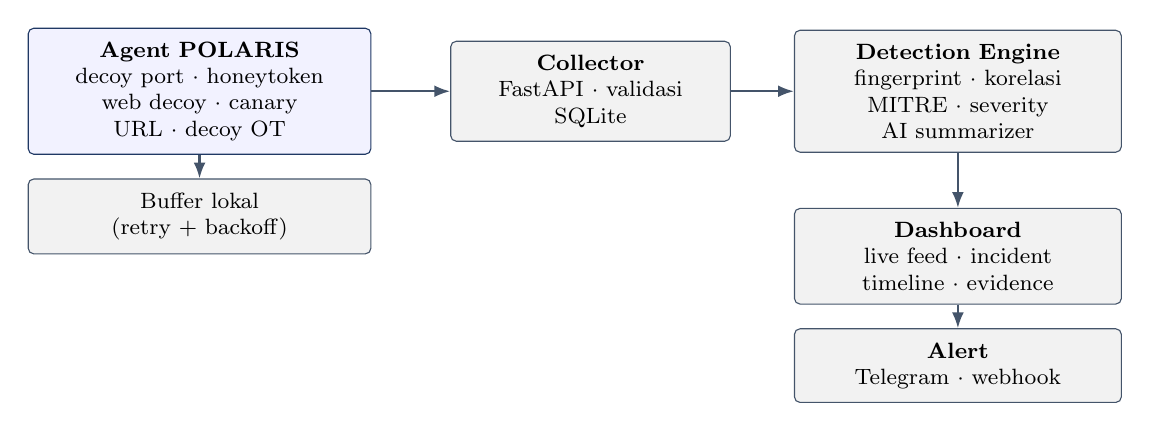
\begin{tikzpicture}[font=\footnotesize,
 box/.style={draw=slate, rounded corners=2pt, fill=lightgray, align=center, inner sep=5pt, minimum height=0.8cm},
 agent/.style={draw=navy, rounded corners=2pt, fill=blue!5, align=center, inner sep=5pt},
 arrow/.style={-{Latex[length=2mm]}, thick, draw=slate}]
\node[agent, text width=4.0cm] (agent) {\textbf{Agent POLARIS}\\decoy port \(\cdot\) honeytoken\\web decoy \(\cdot\) canary\\URL \(\cdot\) decoy OT};
\node[box, below=0.3cm of agent, text width=4.0cm] (buffer) {Buffer lokal\\(retry + backoff)};
\node[box, right=1.0cm of agent, text width=3.2cm] (collector) {\textbf{Collector}\\FastAPI \(\cdot\) validasi\\SQLite};
\node[box, right=0.8cm of collector, text width=3.8cm] (engine) {\textbf{Detection Engine}\\fingerprint \(\cdot\) korelasi\\MITRE \(\cdot\) severity\\AI summarizer};
\node[box, below=0.7cm of engine, text width=3.8cm] (dashboard) {\textbf{Dashboard}\\live feed \(\cdot\) incident\\timeline \(\cdot\) evidence};
\node[box, below=0.3cm of dashboard, text width=3.8cm] (alert) {\textbf{Alert}\\Telegram \(\cdot\) webhook};
\draw[arrow] (agent) -- (buffer);
\draw[arrow] (agent.east) -- (collector.west);
\draw[arrow] (collector) -- (engine);
\draw[arrow] (engine) -- (dashboard);
\draw[arrow] (dashboard) -- (alert);
\end{tikzpicture}}
\caption{Arsitektur POLARIS: agent pada node target, collector, detection engine, dashboard, dan kanal alert.}
\label{fig:arsitektur}
\end{figure}
\subsection{Agent}

Agent ditulis dalam Go dan dikompilasi menjadi satu binary statis. Pilihan ini memberi tiga keuntungan: tidak ada dependensi runtime di server target, cross-compile ke Linux/Windows/ARM mudah, dan goroutine cukup ringan untuk menjalankan beberapa listener sekaligus.

Modul agent dipisahkan berdasarkan jenis umpan: \texttt{decoy/ports.go} untuk listener port, \texttt{decoy/files.go} untuk honeytoken file dan pemantauan filesystem, \texttt{decoy/web.go} untuk jalur web dan login palsu, serta \texttt{decoy/ot\_modbus.go} untuk decoy Modbus/TCP. Modul \texttt{sender} mengirim event ke collector, sedangkan \texttt{buffer} menyimpan event sementara ketika collector tidak tersedia.

Agent berjalan dengan hak akses minimal. Port di atas 1024 dipakai secara default; jika sebuah decoy harus memakai port rendah, agent dapat diberi capability \texttt{CAP\_NET\_BIND\_SERVICE} alih-alih root penuh. Agent tidak menulis ke data produksi dan tidak pernah menjalankan payload yang diterimanya.

Konfigurasi agent dibaca dari file dan environment. Setiap agent memiliki token sendiri untuk mengirim event. Buffer lokal memakai file append-only dengan batas ukuran dan retensi sehingga event tidak hilang saat collector down, tetapi juga tidak memenuhi disk tanpa kendali.

\subsection{Collector dan Detection Engine}

Collector adalah layanan FastAPI dengan tiga endpoint utama: \texttt{POST /ingest} untuk menerima event agent, \texttt{GET /beacon/\{token\}} untuk honeytoken URL, dan \texttt{WS /live} untuk stream ke dashboard. Pydantic memvalidasi payload, token per-agent mengautentikasi pengirim, dan pembatasan laju mencegah banjir event. Data disimpan di SQLite melalui \texttt{aiosqlite}; skema tabel mencakup event, incident, evidence, agent, dan audit log.

Detection engine berjalan sebagai modul Python di dalam collector atau sebagai proses terpisah. Modul \texttt{fingerprint.py} menebak alat penyerang, \texttt{correlate.py} membentuk incident, \texttt{mitre.py} memetakan teknik, \texttt{severity.py} menghitung skor, dan \texttt{summarize.py} menghasilkan narasi opsional. Pemisahan ini memudahkan pengujian unit dan penggantian komponen tanpa mengubah agent.

\subsection{Dashboard dan Kanal Alert}

Dashboard menampilkan live feed melalui WebSocket, kartu incident dengan severity dan teknik MITRE, profil penyerang, timeline, serta bukti. Tampilan utama dibuat sederhana agar dapat dibaca pada layar proyektor saat demo. Kanal alert mendukung Telegram Bot API dan webhook generik; Discord disediakan sebagai opsi. Untuk jaringan air-gap, alert dapat diarahkan ke webhook SOAR internal atau ditampilkan di dashboard lokal.

\subsection{Model Deployment}

Ada tiga model penyebaran. \textbf{Standalone} menempatkan agent, collector, dan dashboard pada satu mesin; cocok untuk demo dan satuan kecil. \textbf{Distributed} menempatkan banyak agent pada node berbeda dengan satu collector/engine pusat; cocok untuk jaringan satuan dengan beberapa server. \textbf{Air-gapped} menjalankan seluruh komponen tanpa internet, dengan paket installer offline dan alert melalui webhook internal atau dashboard lokal.

Instalasi dirancang satu baris: \texttt{curl -fsSL <url>/install.sh | bash}. Untuk air-gap, paket yang sama disediakan sebagai arsip offline. Agent dipasang sebagai layanan sistem, collector dijalankan sebagai service, dan konfigurasi disimpan di direktori terpisah dari data.

\subsection{Keamanan Sistem}

Setiap agent memiliki token sendiri. Collector memvalidasi skema payload, membatasi laju, dan menolak event dari token yang tidak dikenal. Kredensial umpan bersifat inert: tidak memberikan akses nyata dan tidak pernah dipakai untuk autentikasi ke sistem produksi. Agent tidak melakukan tindakan destruktif; auto-block hanya tersedia sebagai opsi yang harus diaktifkan secara eksplisit.

Bukti disimpan dengan hash SHA-256 dan timestamp yang disinkronkan melalui NTP. Payload yang berpotensi memuat data sensitif diredaksi sebelum disimpan. Kebijakan retensi dapat diatur agar disk tidak penuh dan data pribadi tidak tersimpan lebih lama daripada yang diperlukan.

\subsection{Kinerja dan Skalabilitas}

Agent tidak menyimpan state percakapan dengan collector sehingga dapat di-scale horizontal. Collector menyimpan state di SQLite untuk demo; untuk produksi, roadmap menyediakan PostgreSQL. Korelasi berbasis jendela waktu dapat dipartisi per satuan atau tenant. Target kinerja---latensi, overhead, dan throughput---diukur pada lingkungan uji dan dilaporkan apa adanya, bukan diasumsikan.

% ================= 5. METODE PENGEMBANGAN DAN EVALUASI =================
\section{Metode Pengembangan dan Evaluasi}

\subsection{Pendekatan Pengembangan}

Pengembangan memakai siklus prototipe iteratif dalam empat minggu: menetapkan kebutuhan, merancang, membangun, menguji, lalu mendokumentasikan. Setiap akhir minggu menghasilkan artefak yang dapat diuji, bukan hanya catatan desain. Prioritas diberikan pada jalur end-to-end lebih dulu---agent, collector, alert---sebelum memperluas jenis umpan.

\subsection{Lingkungan Uji}

Pengujian dilakukan di laboratorium terisolasi yang terdiri dari dua laptop atau mesin virtual: satu sebagai server target yang menjalankan agent, collector, dan dashboard; satu sebagai mesin penyerang yang menjalankan nmap, hydra, curl, dan klien Modbus. Kedua mesin terhubung melalui switch atau hotspot lokal tanpa akses internet. Snapshot VM disiapkan agar lingkungan dapat direset sebelum setiap skenario.

Tidak ada jaringan operasional TNI AD yang dipakai. Semua data yang dihasilkan adalah data sintetis dari skenario uji. Jika pengujian memerlukan kredensial, yang dipakai adalah kredensial umpan yang inert, bukan kredensial nyata.

\subsection{Skenario Uji}

Pengujian tidak hanya menjalankan serangan. Skenario baseline jinak sama pentingnya karena di situlah false positive muncul.

\begin{table}[htbp]
\centering
\caption{Skenario uji terkontrol}
\label{tab:skenario}
\footnotesize
\begin{tabularx}{\textwidth}{@{}l X X@{}}
\toprule
\textbf{Kode} & \textbf{Aksi} & \textbf{Hasil yang diharapkan} \\
\midrule
S0 & Backup, pembaruan paket, monitoring, dan pemindai kerentanan internal & Tidak ada incident Critical; setiap sentuhan yang tidak disengaja dicatat sebagai kandidat false positive \\
S1 & \texttt{nmap -sV} ke server target & Event T1046, fingerprint mengarah ke nmap atau unknown \\
S2 & \texttt{curl} ke \texttt{/.env}, \texttt{/.git/config}, \texttt{/wp-admin} & Event T1595, alert web decoy \\
S3 & \texttt{hydra} ke decoy SSH & Event T1110, alert brute force \\
S4 & Membaca \texttt{.env} dan \texttt{credentials.txt} umpan & Event T1552.001/T1005, severity High--Critical \\
S5 & Modbus read dan write ke decoy 502 & Event T0886/T0831, alert OT \\
S6 & S1--S3 dari satu IP dalam 15 menit & Satu incident terkorleasi, bukan tiga alert terpisah \\
\bottomrule
\end{tabularx}
\end{table}

\subsection{Metrik Evaluasi}

\begin{table}[htbp]
\centering
\caption{Metrik evaluasi dan target awal}
\label{tab:metrik}
\footnotesize
\begin{tabularx}{\textwidth}{@{}l X l@{}}
\toprule
\textbf{Metrik} & \textbf{Definisi} & \textbf{Target awal} \\
\midrule
Latensi deteksi & Waktu dari event diterima sampai incident tampil atau alert terkirim & \(<5\) detik di LAN \\
Kelengkapan event & Persentase field wajib yang terisi & 100\% field inti \\
False positive & Incident Critical/High pada skenario S0 & 0 Critical/High; kandidat lain didokumentasikan \\
Akurasi korelasi & S6 menghasilkan satu incident, bukan alert terpisah & Satu incident \\
Akurasi fingerprint & Top-1/top-3 tebakan alat & Top-3 untuk alat umum; ``unknown'' diizinkan \\
Overhead & CPU dan RSS agent saat idle dan saat scan & \(<5\%\) CPU; \(<100\) MB RSS \\
Waktu instalasi & Fresh VM sampai agent dan collector berjalan & \(<5\) menit \\
Kelengkapan bukti & Incident memiliki timeline, hash, dan MITRE & 100\% incident \\
\bottomrule
\end{tabularx}
\tabnote{Semua angka adalah target awal yang akan diukur pada lingkungan uji. Tabel ini bukan laporan hasil.}
\end{table}

\subsection{Prosedur Analisis}

Analisis dilakukan secara deskriptif. Setiap skenario dijalankan minimal tiga kali, lalu dicatat latensi, jumlah event, jumlah incident, dan kelengkapan bukti. Karena jumlah skenario kecil dan lingkungan bersifat laboratorium, hasilnya tidak digeneralisasi secara statistik ke jaringan operasional. Penyimpangan dari target dilaporkan sebagai temuan, bukan disembunyikan.

\subsection{Etika dan Keamanan Pengujian}

Pengujian hanya dilakukan pada laboratorium milik penulis. Tidak ada payload destruktif, eksploitasi nyata, atau penggunaan kredensial produksi. Jaringan uji diisolasi dari internet dan dari jaringan kampus atau kantor. Data yang dikumpulkan diminimalkan: event yang tidak diperlukan untuk evaluasi tidak disimpan. Jika pengujian menemukan kerentanan pada perangkat lunak pihak ketiga, temuan dilaporkan secara bertanggung jawab, bukan dipublikasikan tanpa koordinasi.

% ================= 6. RELEVANSI DAN MANFAAT =================
\section{Relevansi dan Manfaat untuk TNI AD}

\subsection{Kebutuhan IT/OT}

Satuan TNI AD mengoperasikan server administratif, layanan internal, dan---di beberapa titik---perangkat OT yang mendukung fasilitas, utilitas, atau komando. Serangan terhadap OT tidak selalu berdampak pada data; ia dapat mengganggu proses fisik. POLARIS menyentuh dua domain itu dengan satu model data: event dari port, berkas, kredensial, dan URL diperlakukan sama seperti event dari decoy Modbus atau HMI. Analis tidak perlu membuka dua sistem terpisah untuk melihat satu sumber yang sama.

\subsection{Kesesuaian dengan Jaringan Air-Gap}

Banyak solusi komersial mengandalkan cloud, langganan threat intelligence, atau konektivitas ke vendor. Di jaringan yang terisolasi, ketergantungan itu menjadi penghalang. POLARIS dirancang dengan dependensi minimal: agent Go, collector Python, SQLite, dan dashboard lokal. Tidak ada fitur inti yang memerlukan internet. AI summarizer bersifat opsional dan dapat diganti dengan template atau model lokal.

\subsection{Pengurangan Beban Analis}

POLARIS tidak menghapus IDS atau SIEM. Ia mengurangi salah satu sumber beban: alert mentah yang tidak memiliki konteks. Event dari umpan dikorelasikan menjadi incident sehingga analis menerima satu kartu yang berisi sumber, timeline, teknik, dan bukti. Jumlah alert yang lebih sedikit dengan kualitas konteks yang lebih tinggi memberi ruang bagi analis untuk menangani insiden yang benar-benar membutuhkan perhatian.

\subsection{Kesiapan Forensik}

Setiap incident menyimpan bukti sejak event pertama: timestamp, alamat IP, port, potongan payload, hash, dan teknik MITRE. Bukti ini belum menggantikan proses forensik formal, tetapi mengurangi pekerjaan awal saat investigasi dimulai. Untuk organisasi yang sering kekurangan log terpusat, kemampuan menyimpan bukti di titik umpan memiliki nilai praktis.

\subsection{Roadmap Adopsi}

Adopsi dapat dimulai dari satu server atau satu segmen laboratorium, lalu diperluas ke node lain tanpa mengubah arsitektur. Tahap berikutnya mencakup integrasi ke SIEM/SOAR, PostgreSQL untuk skala lebih besar, dan penambahan protokol OT. POLARIS tidak menuntut penggantian infrastruktur yang sudah ada; ia menambah lapisan sensor dan analitik di atasnya.

% ================= 7. KELAYAKAN IMPLEMENTASI =================
\section{Kelayakan Implementasi}

\subsection{Stack dan Dependensi}

Agent memakai Go dan pustaka \texttt{fsnotify} untuk pemantauan berkas. Collector dan engine memakai Python dengan \texttt{fastapi}, \texttt{uvicorn}, \texttt{pydantic}, \texttt{httpx}, dan \texttt{aiosqlite}. Dashboard memakai WebSocket dan JavaScript tanpa build tool berat. Database SQLite dipilih karena embedded, tanpa server terpisah, dan cocok untuk jaringan air-gap. Untuk skala lebih besar, roadmap menyediakan PostgreSQL.

\subsection{Instalasi dan Operasi}

Instalasi dirancang satu baris. Agent dipasang sebagai service, collector dijalankan sebagai layanan terpisah, dan konfigurasi disimpan di direktori yang mudah diaudit. Untuk jaringan tanpa internet, paket installer disediakan sebagai arsip offline. Operasi harian mencakup pemeriksaan health check, rotasi log, dan peninjauan incident. Tidak ada ketergantungan pada akun cloud atau lisensi pihak ketiga.

\subsection{Sumber Daya}

Agent berjalan sebagai satu proses dengan listener ringan. Target awal adalah overhead rendah saat idle dan tetap terkendali saat pemindaian; angka pastinya diukur pada evaluasi. Collector dapat berjalan pada satu vCPU dengan RAM terbatas untuk skala demo. Kebutuhan penyimpanan terutama ditentukan oleh retensi event dan bukti, yang dapat diatur.

\subsection{Risiko Implementasi}

Risiko utama bukan teknologi, melainkan penempatan umpan. Umpan yang diletakkan di lokasi yang sering tersentuh backup atau pemindai akan menghasilkan noise. Karena itu, instalasi menyertakan panduan penempatan, allowlist, dan daftar periksa sebelum umpan diaktifkan. Risiko lain adalah kurangnya waktu untuk menguji semua protokol OT; MVP dibatasi pada Modbus/TCP dan HMI web.

% ================= 8. INOVASI TEKNIS =================
\section{Inovasi Teknis}

Kebaruan POLARIS tidak terletak pada penemuan honeypot. Honeypot sudah lama ada \citep{spitzner2002,provos2007}. Kebaruan yang diklaim bersifat rekayasa integrasi dan operasionalisasi, dan itu pun perlu diuji.

Pertama, POLARIS menyatukan enam vektor umpan---port, berkas, kredensial, URL, jalur web, dan OT---dalam satu model event. Kedua, event tidak berhenti sebagai alert mentah; ia dikorelasikan menjadi incident yang menjelaskan satu sumber dalam satu jendela waktu. Ketiga, fingerprinting memberi konteks tentang alat yang mungkin dipakai, dengan opsi ``unknown'' ketika bukti tidak cukup. Keempat, pemetaan MITRE memakai ATT\&CK Enterprise dan ATT\&CK for ICS sekaligus, dengan tingkat keyakinan yang dibedakan.

Kelima, sistem dirancang air-gap-first: tidak ada fitur inti yang bergantung pada internet. Keenam, AI summarizer ditempatkan sebagai lapisan kenyamanan operator, bukan pengambil keputusan. Ketujuh, proposal ini menyertakan model pengendalian false positive dan rencana evaluasi baseline jinak---sesuatu yang sering hilang dari klaim produk deception.

Dengan batasan itu, inovasi yang diajukan dapat diuji: apakah integrasi multi-vektor benar-benar mengurangi waktu analis, apakah korelasi menghasilkan incident yang lebih berguna daripada alert terpisah, dan apakah decoy OT memberi peringatan yang tidak diberikan sensor IT biasa.

% ================= 9. ROADMAP =================
\section{Roadmap dan Rencana Kerja}

\begin{table}[htbp]
\centering
\caption{Roadmap pengembangan sampai batas submission}
\label{tab:roadmap}
\footnotesize
\begin{tabularx}{\textwidth}{@{}l l X X@{}}
\toprule
\textbf{Fase} & \textbf{Tanggal} & \textbf{Keluaran utama} & \textbf{Kriteria selesai} \\
\midrule
W0 & 25--27 Okt & Proposal final, registrasi, webinar pembekalan 2 & Proposal siap submit; lingkungan uji siap \\
W1 & 28 Okt--3 Nov & Agent decoy SSH, honeytoken file, collector, alert Telegram & Satu event mengalir end-to-end dan alert terkirim \\
W2 & 4--10 Nov & Web decoy, canary credential, decoy Modbus/HMI, dashboard, korelasi & Demo penuh dapat dipamerkan \\
W3 & 11--15 Nov & Installer, dokumentasi, video demo, slide, submission & Submit sebelum 15 November \\
\bottomrule
\end{tabularx}
\end{table}

Milestone W1 adalah titik kritis. Jika jalur end-to-end belum berjalan pada 3 November, ruang lingkup dipangkas: port, berkas, dan alert diprioritaskan; web decoy dan OT dipindahkan ke tahap berikutnya. Keputusan go/no-go dicatat agar tim tidak mengejar fitur yang tidak dapat didemokan.

Risiko jadwal terutama berasal dari pemantauan berkas dan simulator OT. Untuk pemantauan berkas, fallback polling mtime disiapkan bila \texttt{fsnotify} bermasalah. Untuk OT, respons Modbus minimal---menerima koneksi, mencatat function code, membalas register palsu---sudah cukup untuk demo; protokol lain bersifat opsional.

% ================= 10. KESESUAIAN KRITERIA =================
\section{Kesesuaian dengan Kriteria Penilaian}

\begin{table}[htbp]
\centering
\caption{Pemetaan proposal ke kriteria penilaian}
\label{tab:kriteria}
\footnotesize
\begin{tabularx}{\textwidth}{@{}l l X@{}}
\toprule
\textbf{Kriteria (bobot)} & \textbf{Bagian} & \textbf{Bukti yang diajukan} \\
\midrule
Relevansi dan Manfaat (25\%) & 1, 6 & Umpan IT dan OT, air-gap, pengurangan beban analis, kesiapan forensik \\
Inovasi Teknis (25\%) & 3, 8 & Enam vektor umpan, korelasi incident, fingerprinting, MITRE Enterprise dan ICS \\
Fungsionalitas Purwarupa (25\%) & 4, 5, 9 & Jalur end-to-end, skenario uji, metrik, rencana demo \\
Kelayakan Implementasi (15\%) & 7 & Binary Go, FastAPI, SQLite, installer satu baris, paket offline \\
Kualitas Dokumentasi (10\%) & Seluruh dokumen & Arsitektur, metode evaluasi, batasan, lampiran teknis \\
\bottomrule
\end{tabularx}
\end{table}

Proposal ini tidak mengklaim skor tertentu. Tabel di atas menunjukkan bagian yang menjawab setiap kriteria sehingga juri dapat menilai klaim dan buktinya secara langsung. Klaim yang tidak didukung pengukuran diberi label sebagai target atau rencana.

% ================= 11. BATASAN =================
\section{Batasan dan Ancaman Validitas}

\subsection{Sumber False Positive}

Klaim ``false positive rendah'' hanya dapat dipertahankan jika sumber gangguannya disebut. Tabel~\ref{tab:fp} merangkum sumber yang paling mungkin dan kontrol yang disiapkan.

\begin{table}[htbp]
\centering
\caption{Sumber false positive dan kontrol operasional}
\label{tab:fp}
\footnotesize
\begin{tabularx}{\textwidth}{@{}l X X@{}}
\toprule
\textbf{Sumber} & \textbf{Contoh} & \textbf{Kontrol} \\
\midrule
Backup & Job membaca \texttt{.env} atau \texttt{credentials.txt} umpan & Allowlist proses/user, jadwal, tier lebih rendah \\
Antivirus/EDR & Pemindaian berkas umpan & Exclusion direktori umpan atau pencatatan low severity \\
Config management & Alat inventaris membaca konfigurasi & Allowlist, maintenance window \\
Vulnerability scanner & Scan port dan jalur web umpan & Daftarkan scanner, korelasi dengan jadwal pemindaian \\
Kesalahan admin & Membuka berkas atau port yang salah & Tier T2, konteks user, review manual \\
Monitoring agent & Akses berkas untuk metrik & Allowlist proses dan path \\
\bottomrule
\end{tabularx}
\end{table}

\subsection{Keterbatasan Lain}

\textbf{Evasi.} Penyerang berpengalaman dapat mengenali umpan dari banner, timing, atau lokasi. POLARIS mengurangi risiko itu melalui realisme, tetapi tidak menghilangkannya. Jika umpan dikenali, interaksi pertama tetap tercatat; nilai deteksinya menurun, bukan nol.

\textbf{OT.} Decoy OT adalah simulasi protokol, bukan pengganti sensor OT pasif. Ia tidak melihat trafik yang tidak menuju umpan dan tidak mengendalikan perangkat nyata. Penempatan di segmen yang salah dapat menurunkan realisme.

\textbf{Generalisasi.} Pengujian dilakukan di laboratorium dengan skenario sintetis. Hasilnya tidak dapat langsung digeneralisasi ke jaringan operasional yang memiliki volume, latensi, dan kebiasaan pengguna berbeda.

\textbf{Kinerja.} Dokumen ini tidak menyajikan hasil pengukuran. Semua angka pada Tabel~\ref{tab:metrik} adalah target yang akan diuji.

\textbf{AI.} Ringkasan AI dapat keliru atau terlalu umum. Karena itu, AI tidak mengambil keputusan dan setiap ringkasan harus dibaca bersama data incident.

\textbf{Legal dan etika.} Pemasangan umpan pada jaringan nyata memerlukan izin pemilik jaringan. Penelitian ini tidak melakukan pengujian pada jaringan TNI AD atau jaringan pihak lain tanpa izin.

% ================= 12. PENUTUP =================
\section{Penutup}

POLARIS tidak menjanjikan deteksi semua serangan. Ia menjanjikan hal yang lebih sempit tetapi dapat diuji: setiap interaksi dengan umpan yang tidak seharusnya terjadi akan tercatat, dikorelasikan, dan disertai bukti yang cukup untuk diperiksa. Pada jaringan yang menggabungkan IT dan OT, kemampuan itu mengisi celah yang sering tidak terjangkau oleh IDS berbasis anomali.

Proposal ini menyatakan batasnya secara terbuka. False positive tidak diklaim nol. Decoy OT bukan pengganti sensor OT pasif. Fingerprinting bersifat best-effort. Purwarupa belum diuji pada jaringan operasional. Yang diajukan adalah rancangan yang dapat dibangun, diuji, dan diaudit---bukan janji yang tidak dapat diverifikasi.

Langkah berikutnya adalah menyelesaikan MVP end-to-end pada W1, memperluas umpan dan korelasi pada W2, lalu menyiapkan installer, dokumentasi, video, dan slide pada W3. Jika dijalankan sesuai roadmap, POLARIS dapat didemokan sebagai sistem yang bekerja, bukan sekadar konsep.

\section*{Pernyataan Orisinalitas dan Penggunaan Alat Bantu}
\addcontentsline{toc}{section}{Pernyataan Orisinalitas dan Penggunaan Alat Bantu}

Penulis menyatakan bahwa ide, rancangan teknis, dan keputusan dalam dokumen ini merupakan karya penulis. Alat bantu AI digunakan untuk menyunting bahasa, memeriksa konsistensi struktur, dan merapikan format. Seluruh klaim teknis, referensi, dan keputusan rancangan diverifikasi oleh penulis. Tidak ada data, hasil pengukuran, atau temuan yang dihasilkan oleh AI. Dokumen ini adalah proposal solusi dan rencana pengembangan; ia tidak menyajikan hasil pengujian yang belum dilakukan.

\clearpage
\phantomsection
\addcontentsline{toc}{section}{Daftar Pustaka}
\begin{thebibliography}{99}
\small
\setlength{\itemsep}{2pt}

\bibitem[Han et al.(2018)]{han2018}
Han, X., Kheir, N., \& Balzarotti, D. (2018). Deception techniques in computer security: A research perspective. \textit{ACM Computing Surveys}, \textit{51}(4), 1--36. \url{https://doi.org/10.1145/3214305}

\bibitem[Pawlick et al.(2019)]{pawlick2019}
Pawlick, J., Colbert, E., \& Zhu, Q. (2019). A game-theoretic taxonomy and survey of defensive deception for cybersecurity and privacy. \textit{ACM Computing Surveys}, \textit{52}(4), 1--28. \url{https://doi.org/10.1145/3337772}

\bibitem[Spitzner(2002)]{spitzner2002}
Spitzner, L. (2002). \textit{Honeypots: Tracking hackers}. Addison-Wesley.

\bibitem[Provos \& Holz(2007)]{provos2007}
Provos, N., \& Holz, T. (2007). \textit{Virtual honeypots: From botnet tracking to intrusion detection}. Addison-Wesley.

\bibitem[NIST(2020)]{nist80053}
National Institute of Standards and Technology. (2020). \textit{Security and privacy controls for information systems and organizations} (NIST SP 800-53 Rev. 5). \url{https://doi.org/10.6028/NIST.SP.800-53r5}

\bibitem[NIST(2021)]{nist800160}
National Institute of Standards and Technology. (2021). \textit{Developing cyber-resilient systems: A systems security engineering approach} (NIST SP 800-160 Vol. 2 Rev. 1). \url{https://doi.org/10.6028/NIST.SP.800-160v2r1}

\bibitem[NIST(2023)]{nist80082}
National Institute of Standards and Technology. (2023). \textit{Guide to operational technology (OT) security} (NIST SP 800-82 Rev. 3). \url{https://doi.org/10.6028/NIST.SP.800-82r3}

\bibitem[MITRE Corporation(n.d.-a)]{mitre_attack}
MITRE Corporation. (n.d.-a). \textit{MITRE ATT\&CK}. Diakses 25 Oktober 2026, dari \url{https://attack.mitre.org/}

\bibitem[MITRE Corporation(n.d.-b)]{mitre_ics}
MITRE Corporation. (n.d.-b). \textit{MITRE ATT\&CK for Industrial Control Systems}. Diakses 25 Oktober 2026, dari \url{https://attack.mitre.org/techniques/ics/}

\bibitem[Kartika Cyber Hackathon(2026)]{kartika2026}
Kartika Cyber Hackathon. (2026). \textit{Kartika Cyber Hackathon 2026}. \url{https://kartikacyberhackathon.id/}

\end{thebibliography}

\clearpage
\appendix

\section{Pemetaan MITRE ATT\&CK}
\label{app:mitre}

Tabel~\ref{tab:mitre} merangkum pemetaan yang digunakan engine. Kolom keyakinan menggambarkan kuatnya bukti terhadap teknik tersebut, bukan tingkat bahaya. Teknik bertanda ID dari ATT\&CK for ICS ditulis dengan penanda ICS; sisanya berasal dari ATT\&CK Enterprise. Event aktual dapat memicu satu atau beberapa baris sekaligus, dan hasil korelasi menyertakan alasan setiap label.

\begin{table}[htbp]
\centering
\caption{Pemetaan aksi teramati ke teknik MITRE ATT\&CK}
\label{tab:mitre}
\footnotesize
\begin{tabularx}{\textwidth}{@{}p{4.9cm} X l l@{}}
\toprule
\textbf{Aksi teramati} & \textbf{Teknik} & \textbf{ID} & \textbf{Keyakinan} \\
\midrule
Koneksi berulang ke banyak decoy port dalam jendela singkat & Network Service Discovery & T1046 & Tinggi \\
Permintaan berulang ke jalur web decoy & Active Scanning & T1595 & Tinggi \\
Percobaan autentikasi berulang pada decoy login & Brute Force & T1110 & Tinggi \\
Pembacaan berkas honeytoken & Unsecured Credentials: Credentials In Files & T1552.001 & Sedang--Tinggi \\
Pembacaan berkas honeytoken & Data from Local System & T1005 & Sedang \\
Penggunaan canary credential pada layanan & Valid Accounts & T1078 & Tinggi \\
Permintaan ke URL honeytoken & Active Scanning / Exploit Public-Facing Application & T1595 / T1190 & Sedang \\
Penggunaan OTP umpan dari sumber tak dikenal & Valid Accounts & T1078 & Tinggi \\
Koneksi ke decoy Modbus/TCP & Remote Services (ICS) & T0886 & Sedang \\
Percobaan write register Modbus & Manipulation of Control / Modify Parameter (ICS) & T0831 / T0836 & Tinggi \\
Koneksi ke decoy RDP tanpa autentikasi & Remote Services: Remote Desktop Protocol & T1021.001 & Rendah \\
Gabungan beberapa jenis event dari satu IP & Kombinasi teknik sesuai event teramati & banyak & Tinggi \\
\bottomrule
\end{tabularx}
\tabnote{Keyakinan turun jika sumber terdaftar pada allowlist operasional, misalnya pemindai kerentanan yang memiliki jadwal. Baris terakhir bukan teknik tunggal, melainkan hasil korelasi multi-umpan.}
\end{table}

Tiga pengecualian perlu disebut. Pertama, satu koneksi tunggal ke satu port umpan tidak dianggap indikasi Network Service Discovery; pemetaan itu hanya diberikan pada pola multi-port. Kedua, percobaan autentikasi yang berhasil terhadap canary credential dipetakan Valid Accounts dengan keyakinan tinggi karena kredensial tersebut tidak memiliki akses sah. Ketiga, pada event OT, sistem tidak mengklaim bahwa proses industri benar-benar berubah; yang teramati adalah interaksi protokol pada umpan.

\section{Daftar Periksa Penempatan Umpan}
\label{app:checklist}

Noise paling sering berasal dari penempatan umpan yang salah, bukan dari salahnya mesin deteksi. Daftar berikut dilalui sebelum umpan diaktifkan pada node produksi.

\begin{enumerate}[leftmargin=1.2cm,itemsep=2pt,topsep=2pt]
  \item Inventarisasi aset di node yang dituju: layanan berjalan, pengguna yang aktif, dan jadwal operasi rutin.
  \item Kumpulkan identitas sumber sah: akun job backup, host pemindai kerentanan, alat konfigurasi, dan agent monitoring.
  \item Pastikan nama berkas dan nomor port umpan tidak dipakai layanan produksi dan tidak berada di jalur yang dibaca berulang oleh monitoring.
  \item Terapkan allowlist pada collector berdasarkan identitas pada butir kedua, bukan hanya berdasarkan alamat IP.
  \item Gunakan port di atas 1024 secara default; gunakan port rendah hanya dengan capability yang didokumentasikan.
  \item Jalankan skenario baseline jinak (S0) satu siklus penuh sebelum alert Critical diaktifkan, lalu tinjau kandidat false positive yang muncul.
  \item Catat di registry umpan: pemilik, tujuan, tier, tanggal pemasangan, dan masa tinjau ulang.
  \item Tinjau ulang secara berkala: hapus umpan yang tidak lagi relevan dan perbarui allowlist ketika episode, aplikasi, atau peralatan berubah.
\end{enumerate}

Registry umpan disimpan bersama konfigurasi agent dan ikut dalam paket instalasi ulang sehingga pemulihan node tidak meninggalkan umpan yang tidak terdokumentasi.

\end{document}
